\documentclass[10pt,a4paper]{amsart}
\usepackage[margin=19mm]{geometry}
\usepackage{amsmath,amssymb,mathtools}
\usepackage[scr=rsfs,cal=euler]{mathalfa}
\usepackage{xfrac}
\usepackage[unicode,hidelinks,bookmarks=false]{hyperref}
\newcommand{\ie}{i.e.\ }
\newcommand{\cf}{cf.\ }
\newcommand{\resp}{respectively\ }
\newcommand{\Subsection}{\subsection}
\providecommand{\nobreakdash}{\nobreak\hbox{-}}
\setlength{\emergencystretch}{2em}
\multlinegap0pt
\usepackage{tikz}
\usepackage{float}
\usepackage{amssymb}
\newtheorem{proposition}{Proposition}
\title{On plus--one generated arrangements of plane conics}
\author{Artur Bromboszcz, Bartosz Jaros\l awski, Piotr Pokora}
\date{Source: arXiv:2507.23024v4 (CC BY 4.0)}
\begin{document}
\maketitle

\noindent\emph{Source and licence.} On plus--one generated arrangements of plane conics. Version arXiv:2507.23024v4 (CC BY 4.0), distributed by arXiv under the Creative Commons Attribution 4.0 International licence, http://creativecommons.org/licenses/by/4.0/, as recorded in the arXiv licence metadata for this exact version and shown on the abstract page https://arxiv.org/abs/2507.23024v4. Full licence notice: \texttt{licenses/arxiv-2507.23024-CC-BY-4.0.txt}.\par\smallskip

\noindent\textit{Editorial scope.} Counted unit: the article's proposition proposition (source0.tex lines 469--471). The article's complete original proof of it is delivered with it (source0.tex lines 472--500, one \texttt{proof} environment of 29 lines). No mathematics is written, repaired or re-derived: the statement and the proof are the article's own lines, in the article's own notation, and no retained line is substituted or re-flowed.  No further source-local context is needed: every cross-reference of every retained line resolves inside the two delivered spans.  Nothing was omitted from any retained span, so the package carries no omission record.  No retained line contains a citation, so the wrapper carries no bibliography and no bibliography entry.  The retained lines contain the article's own diagram code, which the wrapper typesets with the standard tikz packages; no image file is delivered and the package declares no asset dependency.  Editorial formatting only, in addition: an AMS \texttt{amsart} preamble that restates the article's own declarations and macros used by the retained lines, namely the environments \texttt{proposition} on separate counters, together with the standard packages those lines need.  The retained environments print in this document as Proposition 1 in order of appearance, whereas the article prints the same items with the numbering of its own full document.  The complete native source of the article as distributed in the arXiv e-print for this exact version is bundled unchanged as \texttt{sources/182449/source0.tex}.
\begin{proposition}
The combinatorial types $W_{\mathcal{C}_{1}}$ and $W_{\mathcal{C}_{2}}$ of arrangements $\mathcal{C}_{1}$ and $\mathcal{C}_{2}$ are equivalent.
\end{proposition}

\begin{proof}
The arrangements admit only nodes and tacnodes as singularities. A simple inspection, based on the figure below, shows that the combinatorial types of curves $\mathcal{C}_{1}$ and $\mathcal{C}_{2}$ are identical. 
\vskip0.5cm
\begin{figure}[h!]
\begin{minipage}{0.45\textwidth}
\centering
    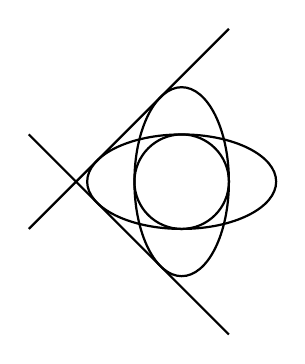
\begin{tikzpicture}[scale=0.6]
\draw[thick] (0,0) circle (1);
\draw[thick] ellipse (2 and 1);
\draw[thick] ellipse (1 and 2);
\draw[thick] (1,-3.2360679774997896964)--(-3.2360679774997896964,1);
\draw[thick] (-3.2360679774997896964,-1)--(1,3.2360679774997896964);
\end{tikzpicture}
\end{minipage} 
\hfill
\begin{minipage}{0.45\textwidth}
\centering
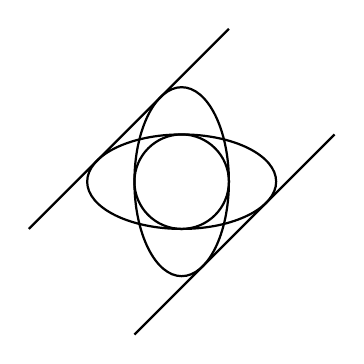
\begin{tikzpicture}[scale=0.6]
\draw[thick] (0,0) circle (1);
\draw[thick] ellipse (2 and 1);
\draw[thick] ellipse (1 and 2);
\draw[thick] (-1,-3.2360679774997896964)--(3.2360679774997896964,1);
\draw[thick] (-3.2360679774997896964,-1)--(1,3.2360679774997896964);
\end{tikzpicture}
\end{minipage}
\label{gr}
\caption{Geometric realizations of arrangements $\mathcal{C}_{1}$ and $\mathcal{C}_{2}$.}
\end{figure}
\end{proof}

\end{document}
